\chapter{Application on real data}
In the simulation we contrasted fixed/updating intercept versions, and in general, both FHTBoost seems to provide a decent model for correlated, realistic survival data, with average deviance much smaller than 0.

\todo[inline]{Make this paragraph better (merge)}

To truly be applicable in biomedical settings, we must see if the algorithm manages to achieve predictive power in a real study.
In this chapter, we consider data from \citet{oberthuer-data}, consisting of data from patients diagnosed with neuroblastoma.
The data consists of a small number of patients, with information on two covariates and around 10 000 gene expressions.
We use FHTBoost on this data and assess its performance.
We also compare the predictive power of our method to Cox regression, specifically CoxBoost, a version of Cox which has been adapted to a boosting framework (see, e.g., \citet{BinderSchumacher2008}), i.e., much like FHTBoost.

\section{Neuroblastoma}
We consider survival data from \citet{oberthuer-data}, consisting of patients diagnosed with neuroblastoma.
Neuroblastoma is a malignant pediatric tumor that accounts for about 8\% of all childhood cancers.
One of the hallmarks of the disease is its contrasting biological behavior, which results in diverse clinical courses ranging from spontaneous regression to rapid and fatal tumor progression despite intensive treatment.

In recent years, several markers have been reported to offer valuable prognostic information.
These markers are routinely determined by the current German neuroblastoma clinical trial NB2004 to stratify patients into groups of high risk (50\%)or low risk (50\%) of disease.
Therapeutic strategies vary according to these risk categories and range from a wait-and-see approach for those in the low risk group,
to intensive treatment for the high-risk group. Still, common clinical experience suggests that such risk classification is still suboptimal for a substantial number of patients.
The individual courses within these risk groups, in particular those of high-risk patients, still vary clearly.

Originally, the data consists of two separate data sets:
A larger training set, collected from Germany, and a smaller test set, collected from several countries.
The training set consists of 256 patients of the German Neuroblastoma Trials NB90-NB2004, where the patients were diagnosed between 1989 and 2004.
%Patients' age at diagnosis ranged from 0 to 296 months, with a median age at 15 months.
%Median follow-up for patients without fatal events was 4.5 years, with a range from 0.8 to 15.6 years.
The test set is an independent set of 120 patients from centers in several countries (including Germany).
In this set, 29 of the samples were obtained from German patients enrolled in German neuroblastoma trials, while the remaining samples are from patients enrolled in national trials in other countries.
%Here the age of patients at diagnosis ranged from 0 to 125 months, with a median at 15 months.
%For patients without fatal events, the median follow-up time was 4.4 years, and ranged from 0.4 to 18.1 years.

Due to few events in the NB2004 low risk group, and following \citet{bovelstad2009}, we merge the ``training set'' and the ``test set'' into one data set.
Hence, in total, the data consists of 362 patients suffering from neuroblastoma.
There are 9978 gene expressions measurements, comprised of those measurements which are in probes from both the ``training set'' and the ``test set.''
From each patient, we have information on their risk group according to the current German neuroblastoma trial as well as the possibly censored survival time.
This survival time was defined as time from diagnosis to first recurrence, and was censored at 5 years.
%Median follow-up time for the patients are 3.8 years.
In addition to the aforementioned risk group, the patient's age at diagnosis is recorded, resulting in two clinical covariates per patient.
89 out of the 362 observations have a missing age.
We remove all of these observations, and are left with a data set of 273.
So $N=273$.
Of these 273, 86 children were classified as having high-risk, while the remaining 187 were not.
It is coded as a binary variable, where both low risk and intermediate risk are coded as 0, and high risk as 1.
42 of the 273 children experienced a recurrence within the follow up, a proportion of 31.5\%.

%\begin{figure}
%\caption{Scatterplot of age in the dataset from \citet{oberthuer-data}.}
%\label{fig:age-scatter}
%\centering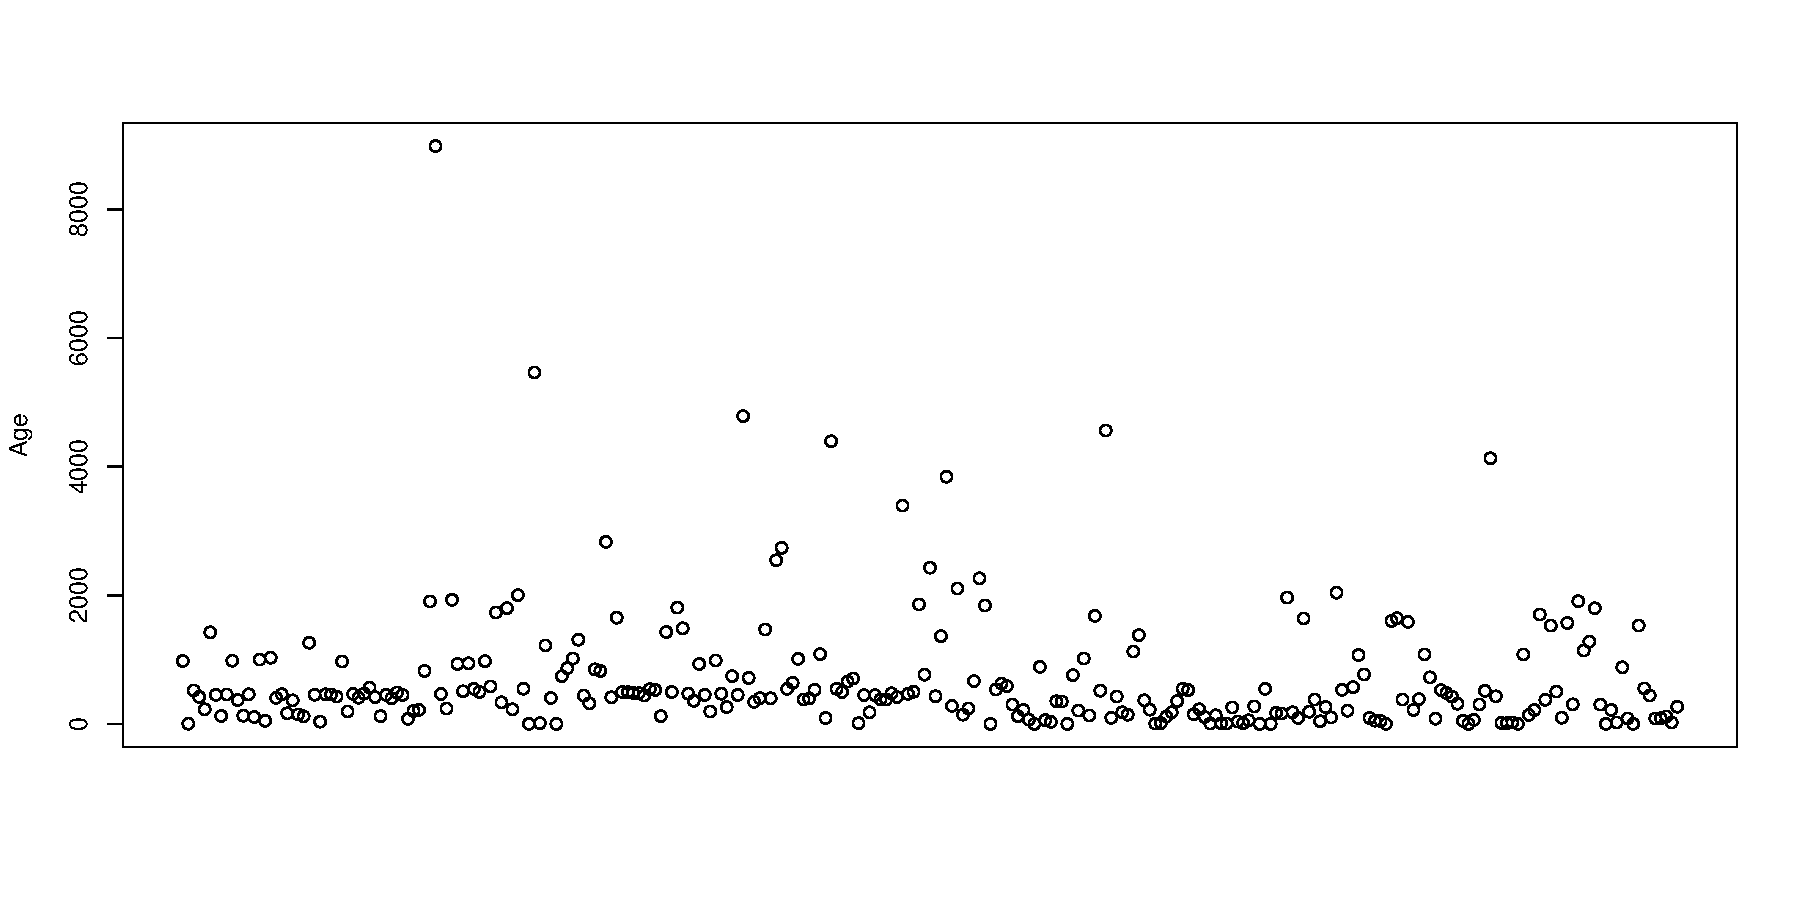
\includegraphics[scale=0.4]{age_scatter.pdf}
%\end{figure}

Due to the lack of data, \citet{bovelstad2009} generated 50 random splits of training and test sets from the merged data set.
We do the same, and generate 100 random splits times.
First, however, we report the analyses of one single (the first) split of train and test data, to give an example of how to interpret the results.

\section{Single split}
We standardize the data to ensure FHTBoost works.
The data are then split in a training set (2/3) and test set (1/3), stratified by the event status.
The training set consists of 182 patients, where 28 are observed events.
The test set consists of 91, where 14 are observed events.

\subsection{Cross-validation on training set}
As has been shown previously, cross-validation should be repeated with different division of folds, as this reduces variance in the estimate of $\mstop$.
We perform a (10 times) repeated 5-fold cross validation to find the optimal number of iterations.
Note in Figure \ref{fig:neuroblastoma-cv} the impact of running the 5-fold cross-validation in a repeated fashion:
Had we used a single 5-fold cross-validation, we would have selected different $\mstop$.
Had either of these been a s the optimal $\mstop$ is different between these different runs.
We first performed a 10-fold repeated cross-validation, but this parameter search did not converge, i.e., the log-likelihood kept increasing.
Upon further inspection, we found that one of the folds was the main cause of this, as the log-likelihood for that particular fold continued to increase, even after 400 iterations, while the other folds were in overfitting territory.
We concluded that splitting a training set of around 180 into 10 folds would eventually cause a problem in one of the folds, as there was too little information left.
We find $\mstop=20$ to be optimal in this case, as shown in Figure \ref{fig:neuroblastoma-cv}.
Each dotted gray line is the sum of the negative log-likelihood of a model trained on 4 folds and applied to the last fold, as a function of iteration number.
The solid black line is the mean of these 10 gray lines, and the red vertical line indicates the optimal $\mstop$, i.e., the minimizing iteration number.

\begin{figure}
\caption{Repeated 5-fold cross validation on training set generated from neuroblastoma data set \citep{oberthuer-data}.}
\label{fig:neuroblastoma-cv}
\centering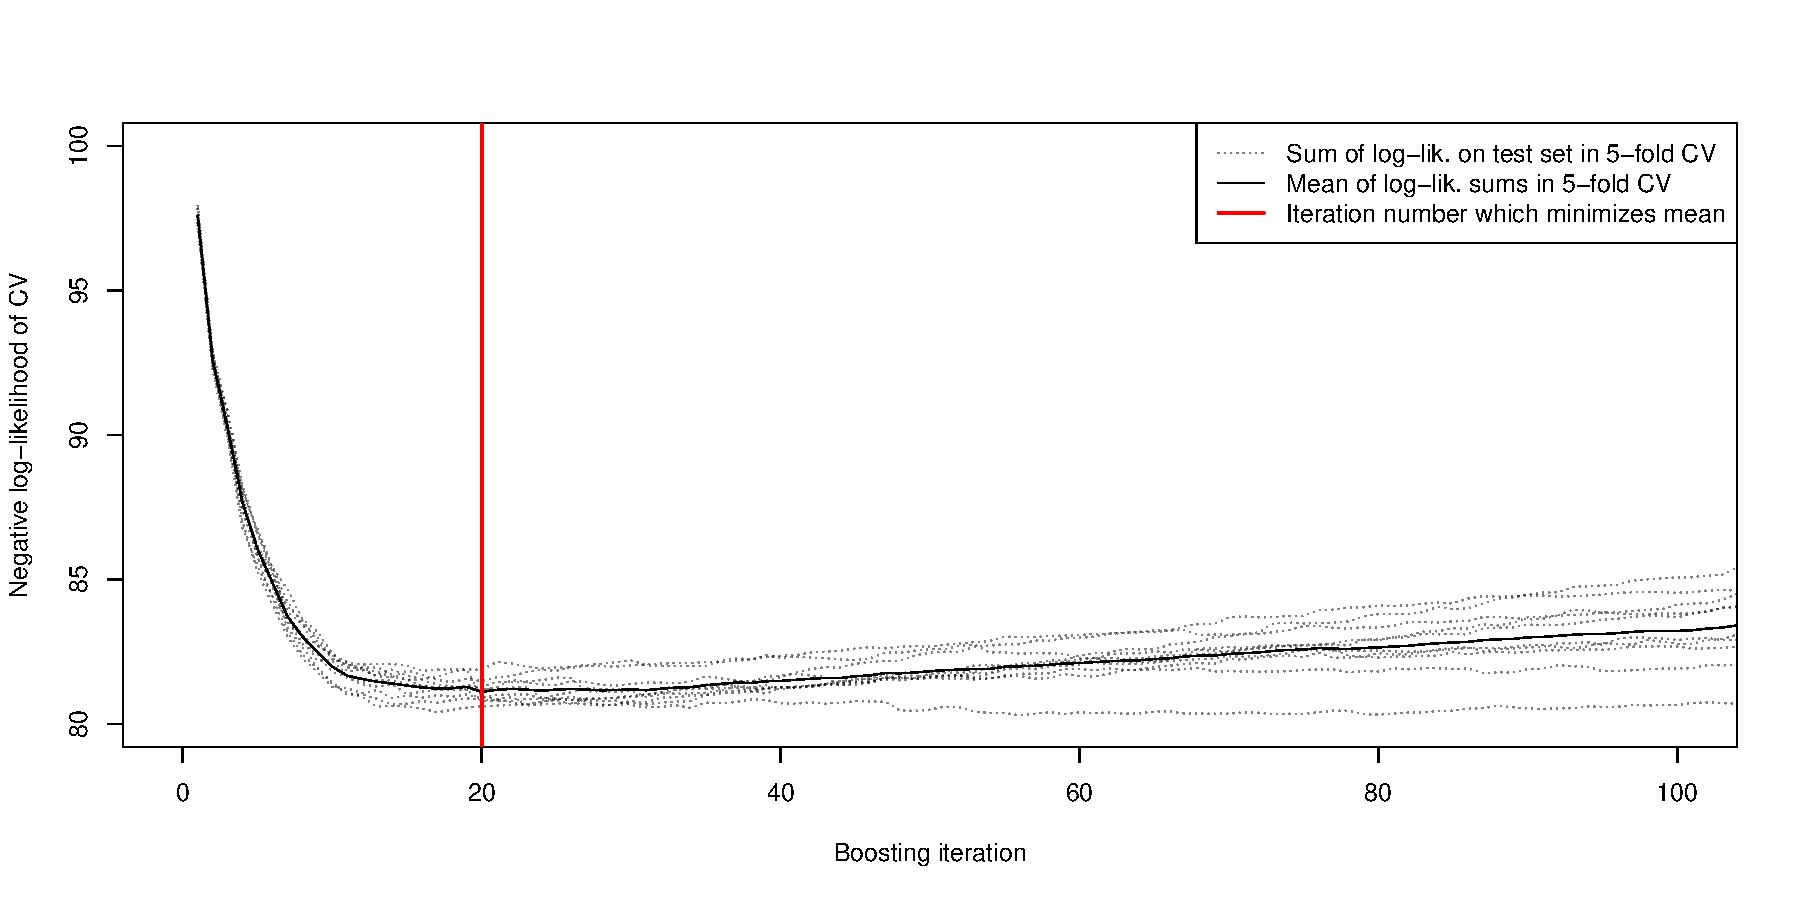
\includegraphics[scale=0.4]{example_cv_loglik.pdf}
\end{figure}

\subsection{Results}
We run the boosting algorithm with $\mstop$ iterations, to estimate the model parameters on the entire training set.

\begin{table}
\caption{Estimated null model on neuroblastoma \citep{oberthuer-data}}
\label{tab:neuroblastoma-intercepts}
\centering
\begin{tabular}{lr}
\toprule
  & Value\\
\hline
$\beta_0$ & 0.692 \\
$\gamma_0$ & 0.077 \\
\bottomrule
\end{tabular}
\end{table}

\subsubsection{Baseline, null model, interpretation}
We first look at the intercepts, reported in Table \ref{tab:neuroblastoma-intercepts}, meaning, the null model parameters.
The estimated intercept for the gene data, $\beta_0$, is 0.692.
We recall that in the FHT model, the vector $\bbeta$ corresponds to the initial level $y_0$ of the health process, with the log link function.
The null model, without any covariate effects, therefore has a $y_0$ of $\exp(0.692)=1.998$.
Further, the intercept for the clinical data is estimated to be 0.077.
This means that the health process with the FHT interpretation that arises from our estimation is a Wiener process with a relatively small initial level of 1.998, and with a \textit{positive} drift, albeit slightly, of 0.077.
Recall also that the Wiener process has a unit variance in each time unit, meaning the variance is equal to the time unit $t$.
The large variability of the process relative to its starting point means there is still a significant chance of recurrence of neuroblastoma.
The resulting health process is
\begin{equation*}
    Y(t)=1.998+W(t)\cdot0.077t,
\end{equation*}
where $W(t)\sim N(0,\sqrt{t})$,
i.e.,
\begin{equation*}
    Y(t)\sim N(1.998+0.077t,\sqrt{t}).
\end{equation*}
To get a feeling of the variability of it, and potential trajectories of such a process, we plot 10 realizations of this process in Figure \ref{fig:neuroblastoma-wien}.
Of these particular 10 processes, 8 processes at some point go below 0.
In the FHT interpretation, then, these health processes would cause a death, or, a recurrence of the neuroblastoma cancer.
To get a better estimate of the proportion of health processes not dying, we need to sample more processes.
We sampled 10000, and 6221 of these went below 0 within $t=40$, i.e., a proportion of 0.378 did not experience recurrence.
In section \ref{sec:FHT}, specifically in equation \eqref{eq:P-inf-FHT}, we stated the probability of an IG FHT lifetime not ending, i.e., the cure rate.
We will have a non-zero cure rate if the drift is positive, like we have here in our null model.
We calculate this for our estimated null model, obtaining
\begin{align*}
    \Pr{(T=\infty)}=1-\Pr{(T<\infty)}&=1-\exp{(-2\cdot y_0^{[0]}\cdot\mu^{[0]})}\\
    &=1-\exp{(-2\cdot 1.998\cdot 0.077)}=0.265,
\end{align*}
meaning about three in four should have a recurrence during their lifetime.
For this training set, 28 out of 182 are observed events, meaning only 0.154 have experienced a recurrence.
Note that this is with a medium follow-up of 4.5 years.
It is, however, still a bit off from the cure rate obtained from the estimated null model, but our model does predict a non-zero proportion of long-term survivors, which is good.
\begin{figure}
\caption{Wiener processes with parameters $y_0=1.998$ and $\mu=0.077$, corresponding to the estimated null model from the neuroblastoma data set \citep{oberthuer-data}.}
\label{fig:neuroblastoma-wien}
\centering
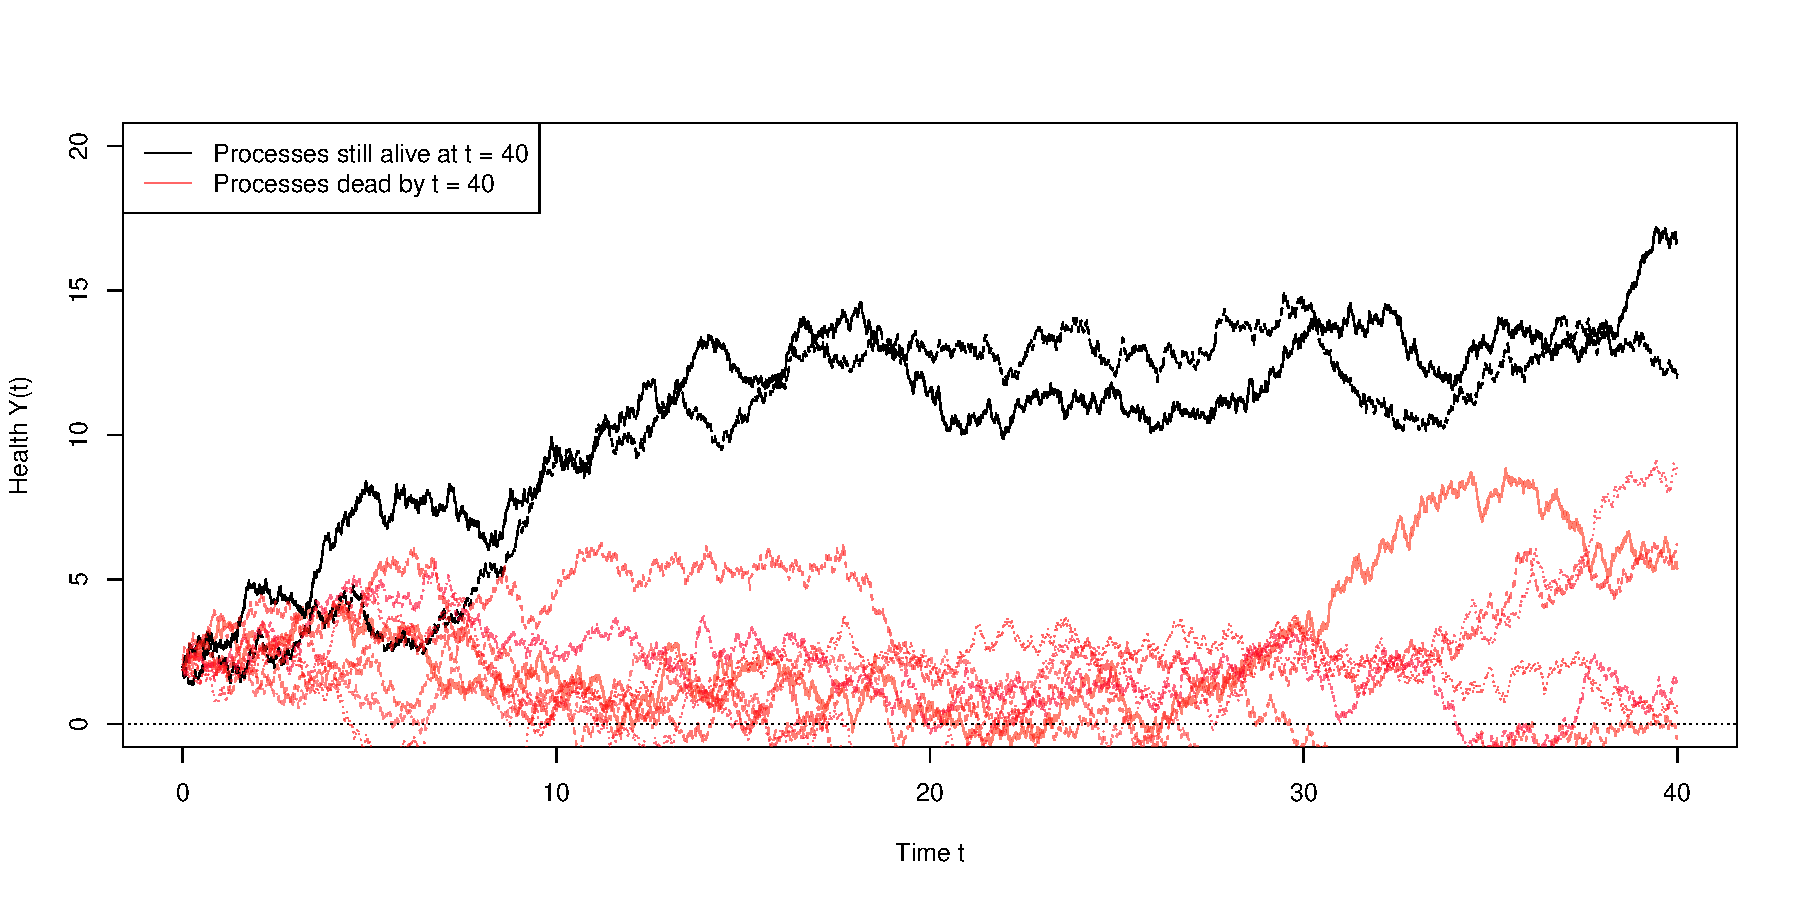
\includegraphics[scale=0.4]{example_wieners.pdf}
\end{figure}

Consider the fact that the initial level $y_0$ is quite low.
Since we are looking at when, if ever, a neuroblastoma patient will have a recurrence after a surgery, this initial level of the Wiener process is the health level of a patient at surgery.
The health of such a child is often presumable quite precarious, as neuroblastoma is a malignant cancer.
Therefore it makes sense that the initial level $y_0$ is quite low.
However, the survival probability of patients vary, as is experienced by clinicians, even among those specified as high-risk.
Most children will, as estimated by our model, survive.

Now consider the fact that the drift $\mu$ is positive.
Since the individuals in the study are young children, and we are looking at a timeframe that does not comprise the length of a typical human life, the health level of most children should indeed increase after the surgery.

\subsubsection{Estimated covariates}
Let us further look at estimated covariate effects (Table \ref{tab:oberthuer-beta} and Table \ref{tab:oberthuer-gamma})
We see that the boosting algorithm has included both covariates into the model.
Before splitting into training and test sets, we centered and scaled each column of the covariate matrices, such that the mean across all individuals is (approximately) 0 for each covariate $j$,
%\begin{equation}
%    \overline{x}_j=\frac{1}{n}\sum_{i=1}^n x_{i,j}\approx 0,
%\end{equation}
and the standard error is approximately 1.
%\begin{equation}
%    s_j=\frac{1}{n}\sum_{i=1}^n (x_{i,j}-\overline{x}_j)^2\approx 1.
%\end{equation}
%(See a previous section for an explanation of why centering and scaling is important.)
For the gene expressions, this is not particularly important with regards to interpretation, as the scale of these do not lend themselves easily to interpretation.
However, to properly consider the interpretation of the estimated parameters corresponding to the clinical measurements, we should
scale these back to their original scale.
For example, the covariate corresponding to risk, namely $\gamma_1$, is originally either 0 or 1, depending on the covariate.
After standardizing, these are -0.677 and 1.472, respectively.
The most striking result here is the large parameter corresponding to risk.
We calculate the drift parameter for those individuals designated as high-risk, and it is
\begin{equation*}
    \mu^{[0]}_{\text{high-risk}}=0.077-0.189\cdot1.472=-0.202.
\end{equation*}
Whereas for those designated as low and intermediate risk, it is
\begin{equation*}
    \mu^{[0]}_{\text{low-risk}}=0.077-0.189\cdot-0.677=0.205.
\end{equation*}
Since age is standardized, these two drift covariates should be the mean drift parameters for each of the groups.
The effect of age is negative, which means that there is some downward effect on the drift as the child's age increases.
This negative effect could also potentially lead to low-risk individuals having an estimated negative drift, if the child is sufficiently old.
This is, however, not the case.
The effect of age is so small as to not impact the sign of the drift.
Because the maximum standardized age is 4.193, the age contribution to drift is bounded below by 
\begin{equation*}
    -0.029\cdot4.193=-0.122.
\end{equation*}
Similarly, there are no high-risk individuals for which the drift will be positive, since the minimum standardized age is -0.724, and so the effect of age is bounded above by
\begin{equation*}
    -0.029\cdot0.724=0.021.
\end{equation*}
Hence, crucially, this means that the model predicts that all high-risk individuals will eventually have a recurrence of neuroblastoma cancer.
This seems to resonate with the fact that these children are indeed characterized as having a high risk of recurrence.
Those not designated as high-risk, on the other hand, have a probability of not experiencing recurrence, using the formula seen previously, namely
\begin{equation*}
    1-\exp{(-2\cdot y_{0}^{[0]}\cdot\mu_{\text{low-risk}}^{[0]})}=1-\exp{(-2\cdot 1.998\cdot 0.205)}=0.559.
\end{equation*}
We should therefore expect, based on the estimated model, that more than half of the low-risk patients should recover.


\begin{table}
\caption{Results of estimated gene coefficients on neuroblastoma data \citep{oberthuer-data}.}
\label{tab:oberthuer-beta}
\centering
\begin{tabular}{lrr}
\toprule
Gene $j$      & $\beta_j$ (full) & $\beta_j$ (genomic only)\\
\hline
Gene 49   & -0.010  &      0  \\
Gene 1447 & -0.069  & -0.047  \\
Gene 3191 &      0  & -0.051  \\
Gene 2442 &  0.012  &      0  \\
Gene 4447 &      0  & -0.062  \\
Gene 5307 &      0  &      0  \\
Gene 5527 & -0.073  & -0.098  \\
Gene 5725 & -0.009  &      0  \\
Gene 6532 & -0.011  &      0  \\
Gene 6701 &  0.015  &      0  \\
Gene 6901 &  0.011  &      0  \\
\bottomrule
\end{tabular}
\end{table}

\begin{table}
\caption{Results of estimated clinical coefficients on neuroblastoma data \citep{oberthuer-data}.}
\label{tab:oberthuer-gamma}
\centering
\begin{tabular}{lrr}
\toprule
Clinical covariate & $\gamma_j$ (full) & $\gamma_j$ (clinical only)\\
\hline
Risk      &  -0.189  &  -0.268\\
Age       &  -0.029  &       0 \\
\bottomrule
\end{tabular}
\end{table}

We observe that 8 genes have been selected in 20 boosting iterations (see Table \ref{tab:oberthuer-beta}).
Some effects are estimated to be positive, some to be negative.
Again, the gene expression measurements have been centered and scaled.
However, a larger parameter does not necessarily mean that the effect of this gene is in general larger than others, as that still depends on the distribution of these.
It is more difficult here to say how much the genomic data helps in explaining the variance.


\subsection{Difference of deviance on the test set}
The test set consists of 91 individuals, of which 14 have experienced recurrence.
With the estimated model, we calculate the deviance, as seen in Section \ref{sec:deviance}.
Recall that the performance of a model is good when the difference in deviance is small (i.e. negative with a large absolute value).
We obtain a difference of deviance on -95.2, which is quite a lot!

\section{Comparing a clinical-genetic model to clinical-only and genetic-only models}
\citet{bovelstad2009} analysed the neuroblastoma data and compared different ways of combining clinical and genomic data in Cox models.
As mentioned in subsection \ref{subsec:FHT-combine}, the FHT model lends itself easily to combining genomic and clinical data.
Our boosting method FHTBoost offers a simple way to combine clinical and genetic data in estimating.
There is also a straightforward way to only use clinical covariates, or to only use genetic covariates.
To do this, we can use the cyclical version of the algorithm, where we booth both parameters in each step, but they have their own tuning parameter.
This lets us fix the number of boosting steps of the parameter not to be boosted to 0.
In other words, a genomic version of FHTBoost, or $y_0$-only version of FHTBoost, where we boost only the initial level $y_0$.
This version of FHTBoost has $m_{\text{stop},1}$, corresponding to $\mu$, fixed at 0, while we perform cross-validation in the usual way to find the optimal $m_{\text{stop},2}$, corresponding to $y_0$.
Similarly, the clinical version fixes $m_{\text{stop},2}$ at 0, and tunes the other, $m_{\text{stop},1}$, corresponding to $\mu$.
In this way, we can compare the performance of our model across the genetic and clinical data, in a similar way as in \citet{bovelstad2009}.

We do the estimation and the test set calculation, and we get the difference of deviance results shown in table \ref{tab:deviances}.
We see here, in fact, that in this case the full model is beaten by the genomic model, with difference of deviance of -95.2 and -104.4, respectively.

\begin{table}
\caption{Difference of deviance results.}
\label{tab:deviances}
\centering
\begin{tabular}{cc}
\toprule
Boosting type & Difference of deviance \\
\hline
Full & -95.2 \\
Clinical ($y_0$) only  & -14.5 \\
Genetic ($\mu$) only & -104.4 \\
\bottomrule
\end{tabular}
\end{table}

Furthermore, we calculate the Brier scores at the time points of the test set.
See Figure \ref{fig:brier-FHT} for a comparison of the Brier score of the three different FHT models.
We see here that, in fact, the genomic model performs best, and quite strikingly so.

\begin{figure}
\caption{Brier scores for FHT models.}
\label{fig:brier-FHT}
\centering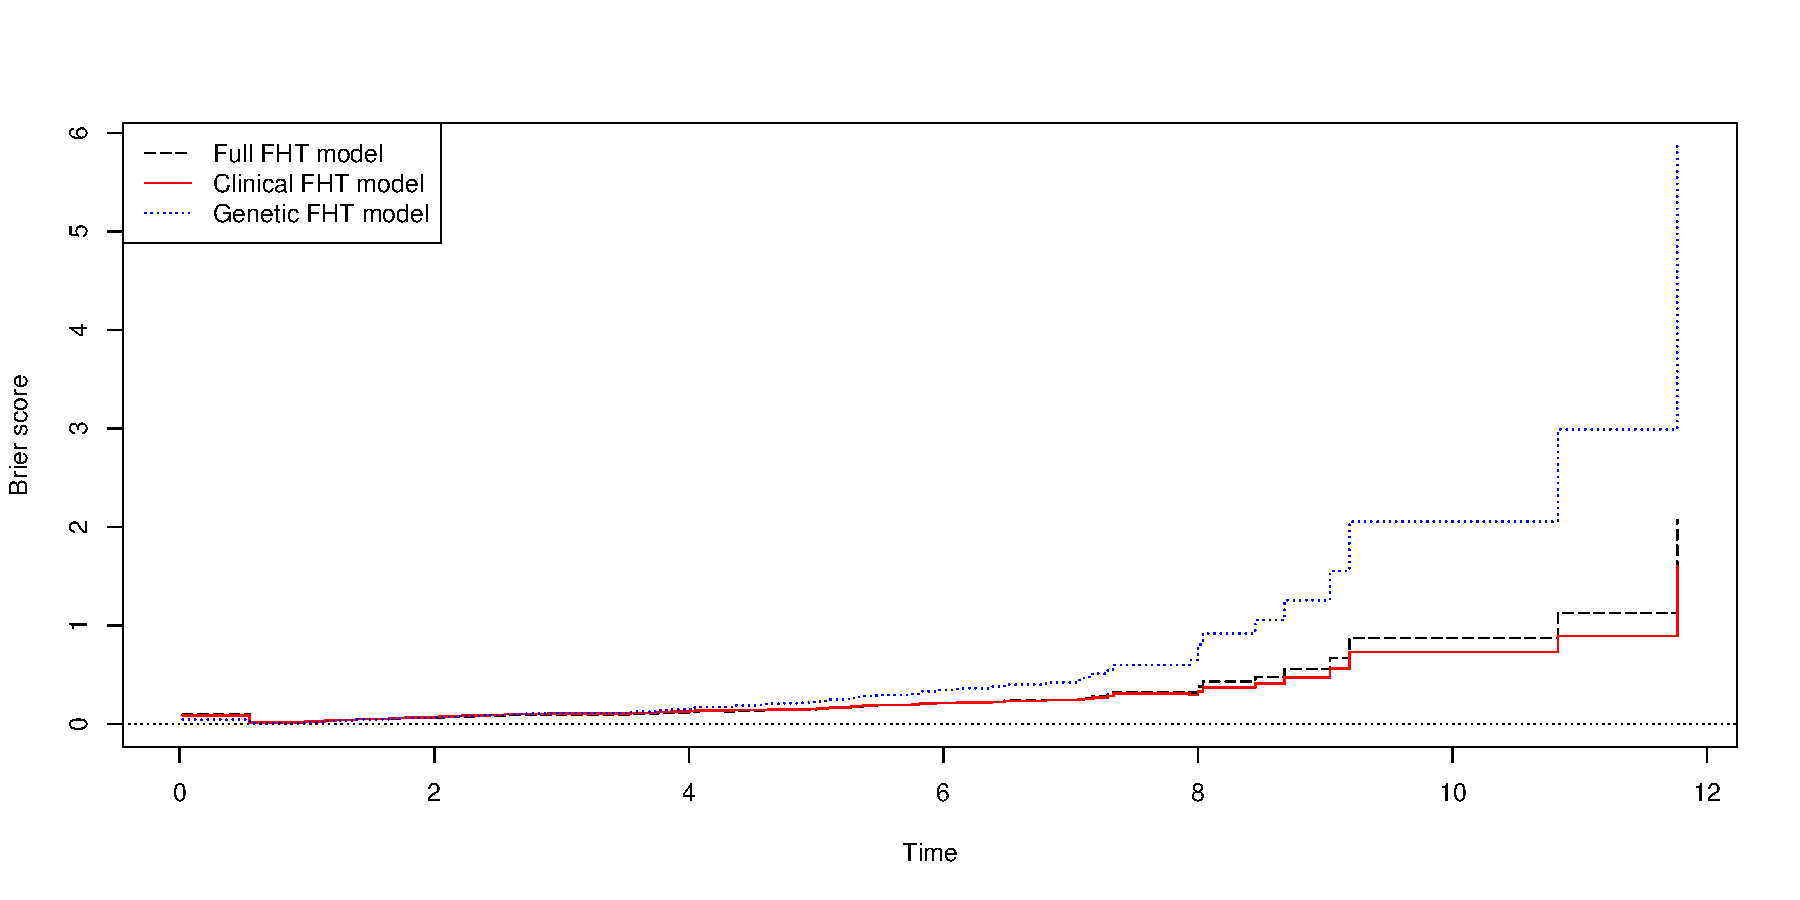
\includegraphics[scale=0.4]{brier_FHT.pdf}
\end{figure}

\section{Comparison with the Cox model}
The Cox model which has been discussed previously, in Chapter 2.
We compared our model with the Cox model as implemented in CoxBoost \citep{...}, setting
\begin{equation}\label{eq:lambda-nu}
    \lambda=N\frac{1-\nu}{\nu},
\end{equation}
as suggested in \citet{DeBin2016}, where $N$ is the number of individuals in the data set on which the estimator is applied, and $\nu$ is the step length mentioned in the various boosting algorithms in chapter \ref{ch:boosting}, which we by convention always set to 0.1.

For the specific case discussed previously, we calculate the Brier score for these models.
Consider now a comparison between the Brier score for the full FHT model and the Cox model, in Figure \ref{fig:brier-cox-both}.
We can see that the Cox model performs better for all times, but the difference in performance also increases over time.
Consider now Figure \ref{fig:brier-cox-genetic}, in which we compare the Cox model to the genomic model.
What is especially interesting here is that the Brier score of the genomic model almost overlaps with the Brier score of the Cox model.
That is, except the positive jumps that the Cox model performs in the beginning, mostly from time 0 to 4.
I do not know why these jumps happen.

\begin{figure}
\caption{Brier scores for Cox and both.}
\label{fig:brier-cox-both}
\centering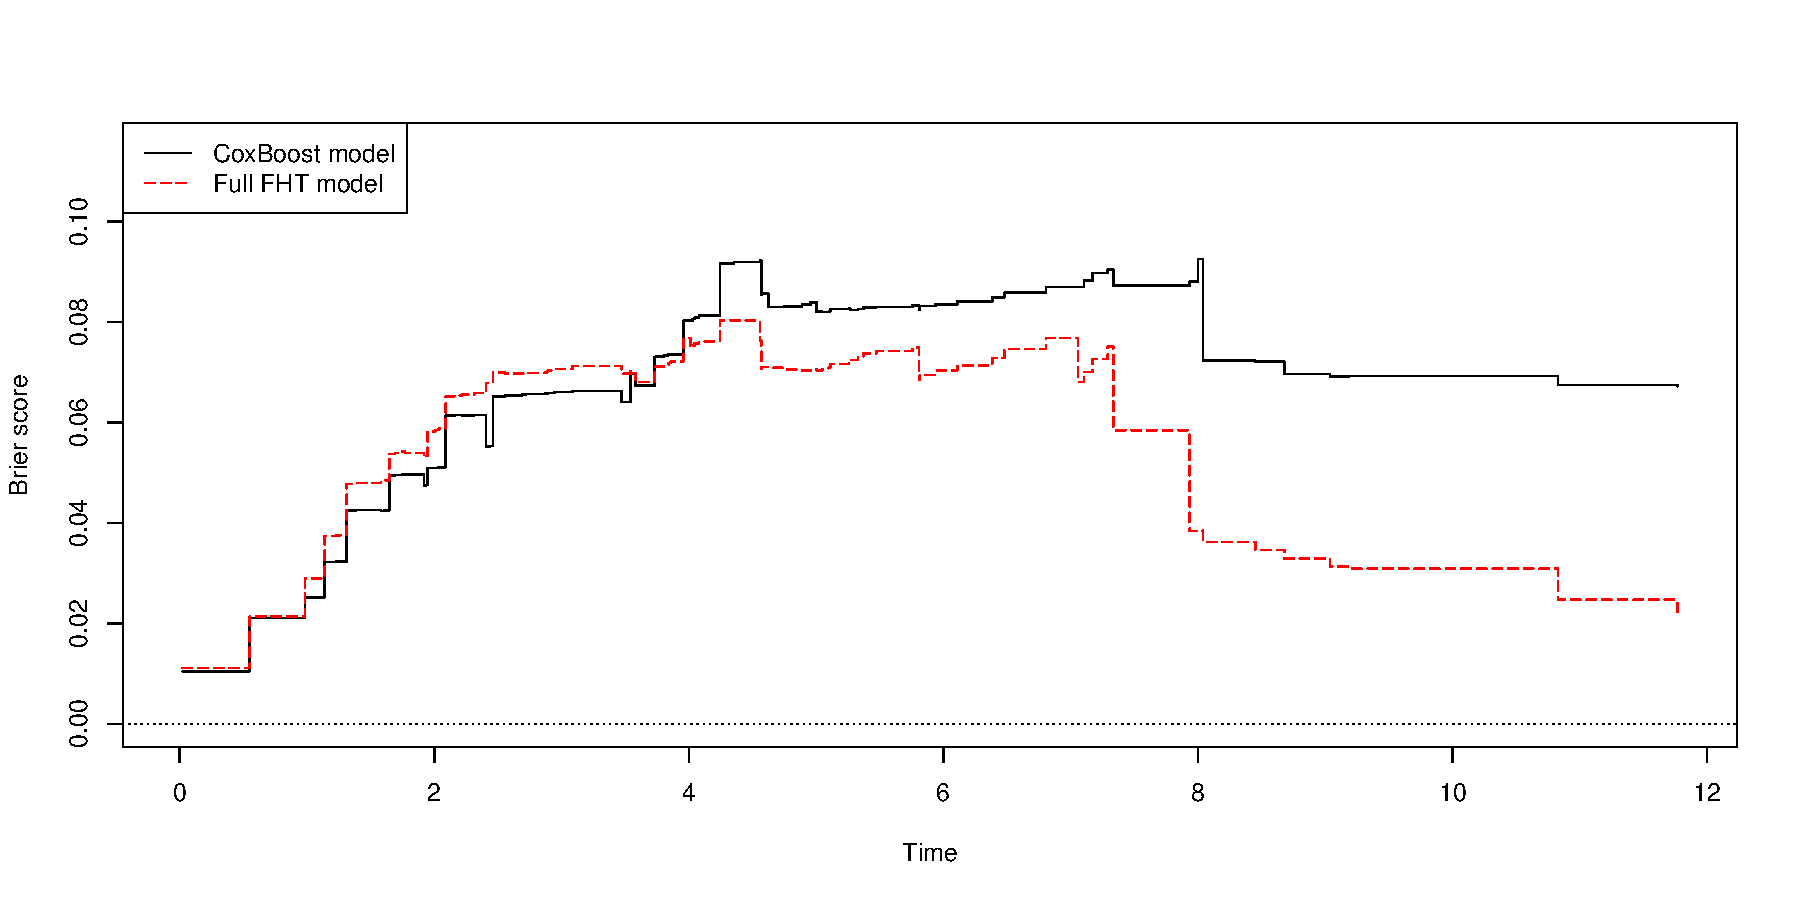
\includegraphics[scale=0.4]{brier_cox_both.pdf}
\end{figure}
See Figure \ref{fig:brier-cox-both} for a comparison of the Brier score of the boosted Cox model and the boosted FHT model.
\begin{figure}
\caption{Brier scores for Cox and genetic FHT model.}
\label{fig:brier-cox-genetic}
\centering
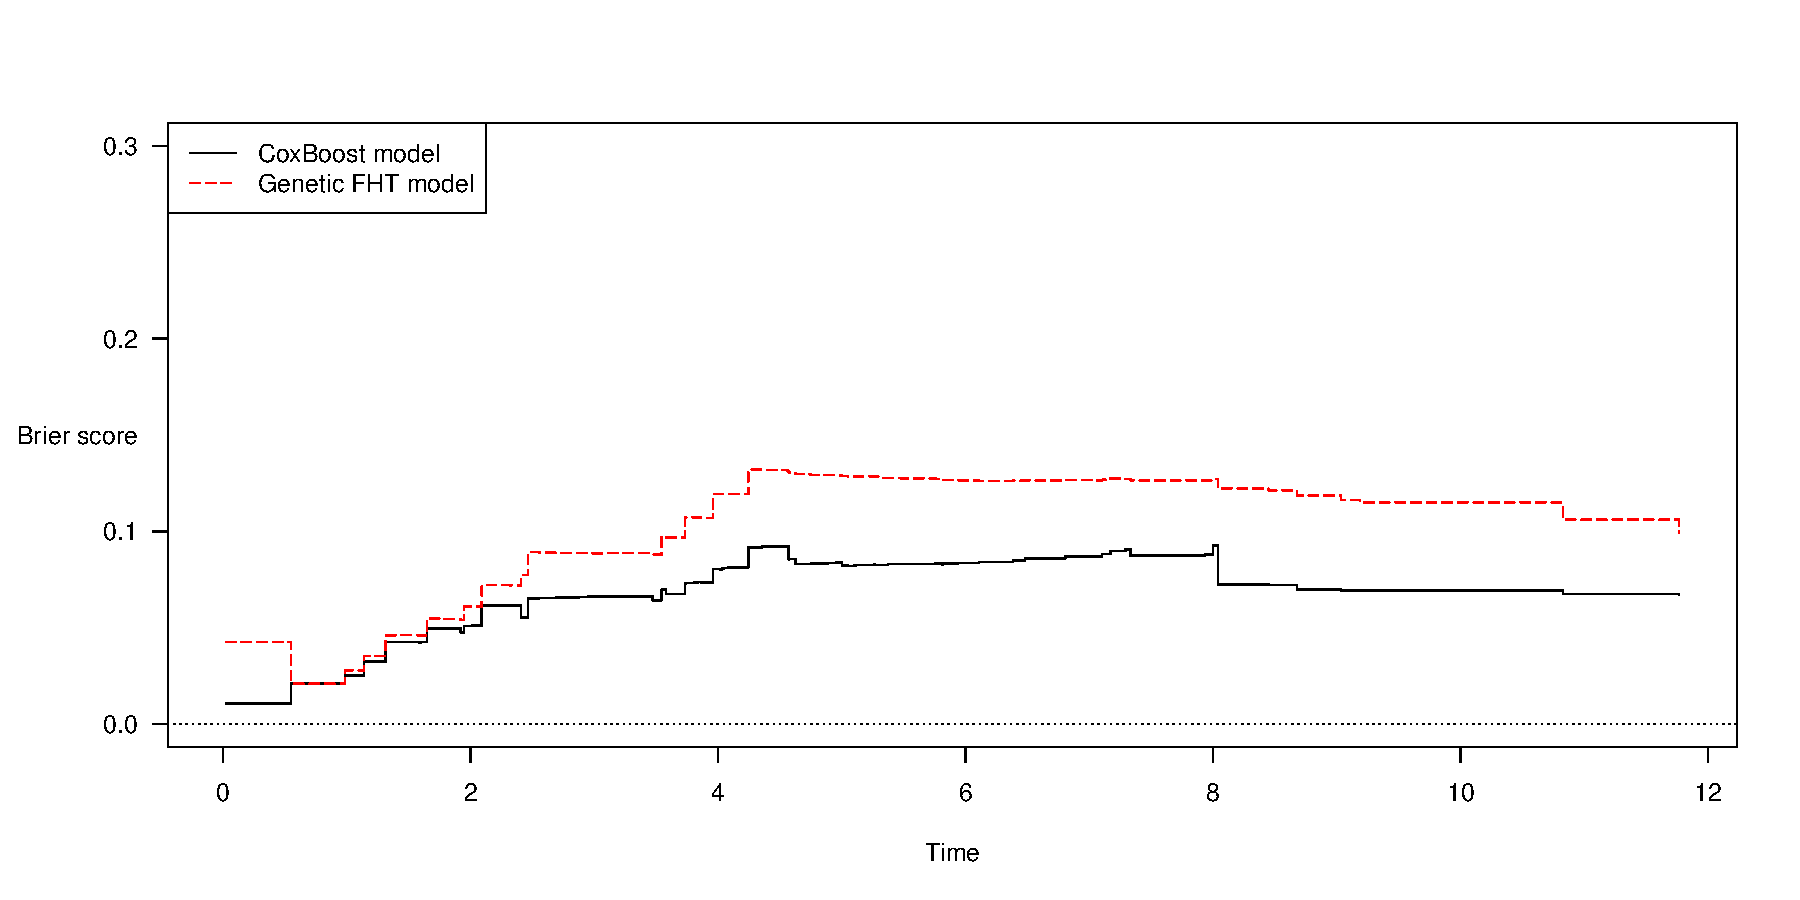
\includegraphics[scale=0.4]{brier_cox_genetic.pdf}
\end{figure}

%\begin{figure}
%\caption{Brier scores for Cox and Cox mandatory model.}
%\label{fig:brier-cox-mandatory}
%\centering
%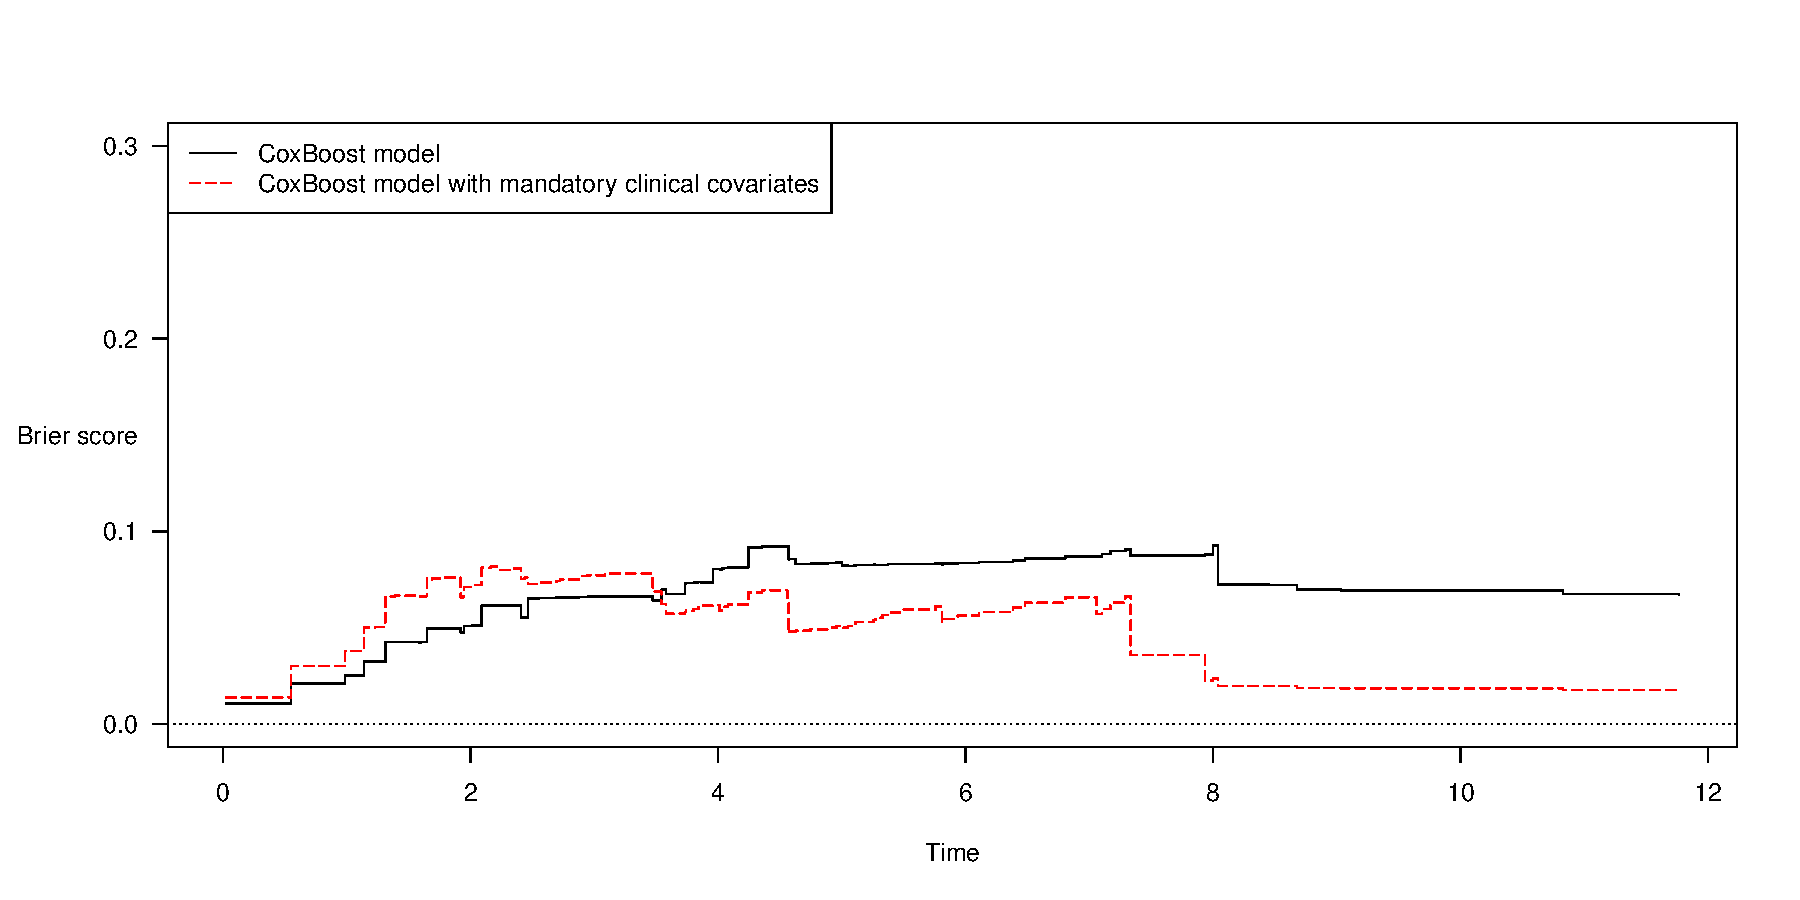
\includegraphics[scale=0.4]{brier_cox_mandatory.pdf}
%\end{figure}

%\todo[inline]{Cite these packages! I think cite(package) in R}


\section{Analysis of 100 train/test splits}
\citet{bovelstad2009} generated 50 random splits of training and test sets from the data, to see the distribution.
We now generate 100 splits of training and test sets, in the same manner.
We use the same method as above.
We first estimate parameters based on the training set, and then calculate the model's difference of deviance, on the test set, using the parameters estimated on the training set.

\subsection{Comparing deviance of FHT models}
We now consider the difference of deviance across all 100 splits of training and test sets.
All 
The 
See Figure \ref{fig:neuroblastoma-deviances} for difference of deviance boxplot.
We use the median of difference of deviance as the main measure of interest.
It is -24.3172 for the full model, and -21.60033 for the clinical model, and 4.009162 for the genomic model.
See Figure \ref{fig:neuroblastoma-deviances} for a boxplot of these.

\begin{figure}
\caption{Boxplot for difference in deviance for different variants of the FHT model.}
\label{fig:neuroblastoma-deviances}
\centering
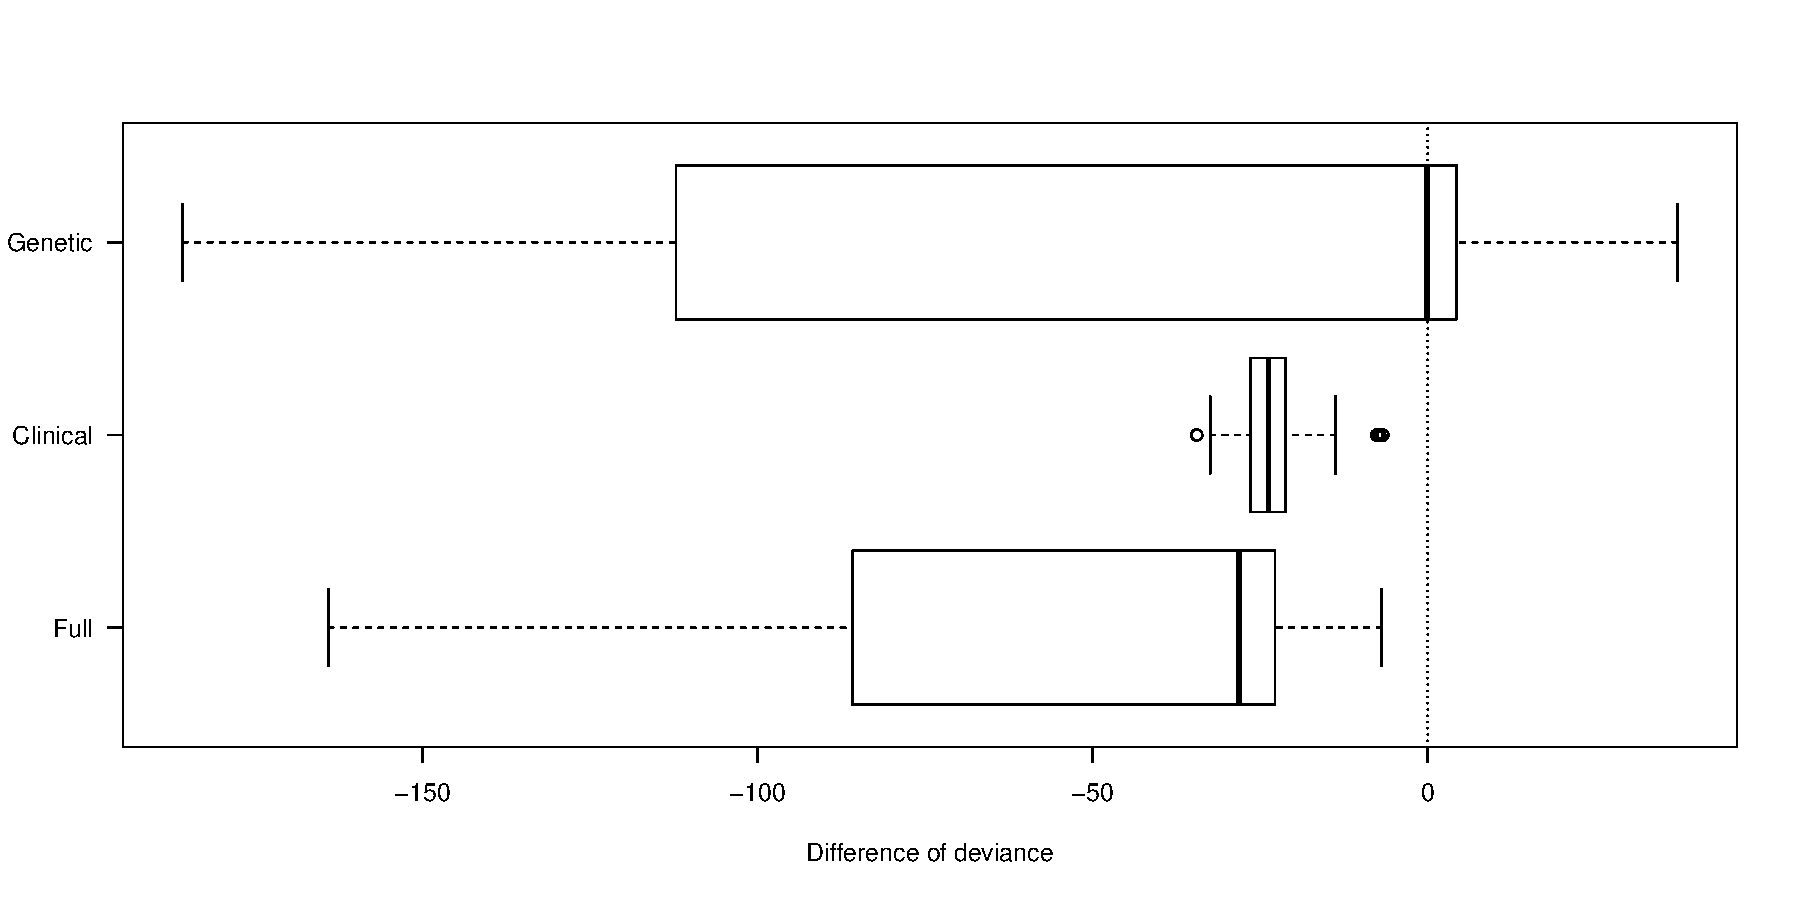
\includegraphics[scale=0.4]{deviance_FHT.pdf}
\end{figure}

These deviances look a bit strange, at least the box for the full model, and the box for the genomic model.
The median looks to be very strangely positioned, all the way to the right of the boxes.
We plot histograms of these two to consider why.
See Figure \ref {fig:neuroblastoma-deviances-histo}.
The reason turns out to be that they are quite bimodal in their distribution.
Both have large peaks around 0, and both have smaller and wider peaks more to the left.
We see that the full model consistently improves performance with covariates, i.e., has a negative difference of deviance.
This resonates with the fact that the clinical model also improves over the null model.
However, the genomic model very often does not improve on the null model.
Although, its most extreme values are in cases where the difference of deviance is very small, and so these are cases where the genomic model outperforms the full model.

\begin{figure}
\caption{Histogram of difference of deviance for the genomic model and the full model.}
\label{fig:neuroblastoma-deviances-histo}
\centering
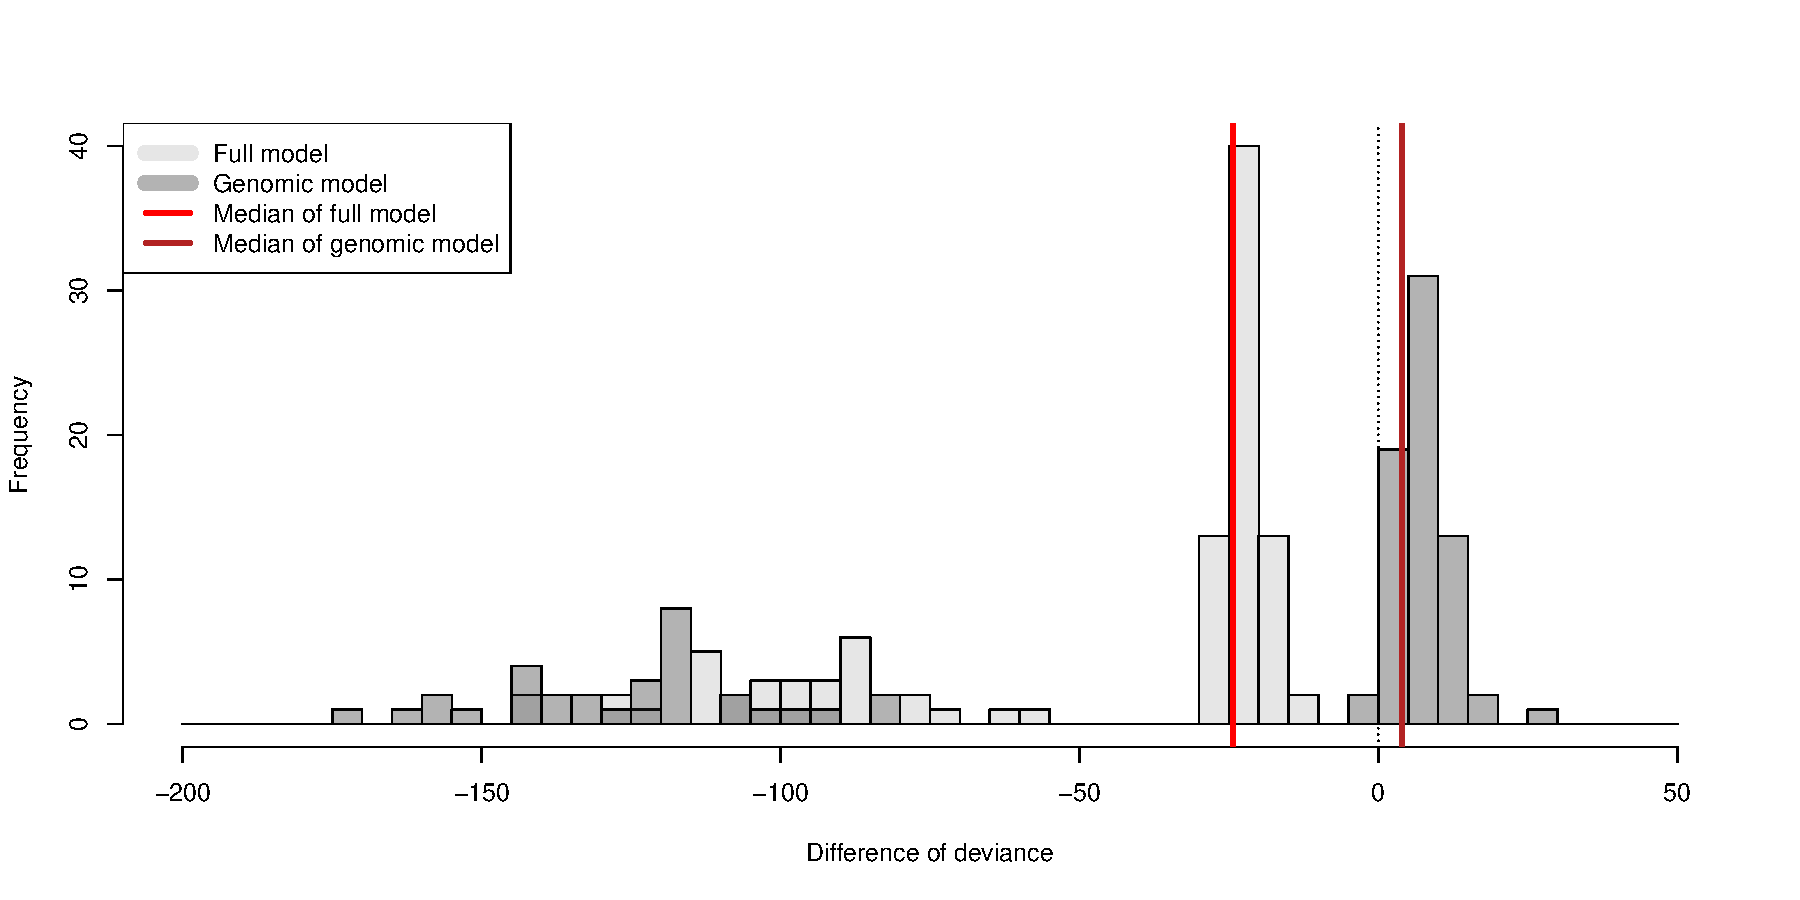
\includegraphics[scale=0.4]{deviances_histogram.pdf}
\end{figure}


\subsection{Integrated Brier scores results}
We now calculate integrated Brier scores for all 100 splits.
A boxplot can be seen in Figure \ref{fig:neuroblastoma-integrated-brier}.
\begin{figure}
\caption{Boxplot of integrated Brier scores.}
\label{fig:neuroblastoma-integrated-brier}
\centering
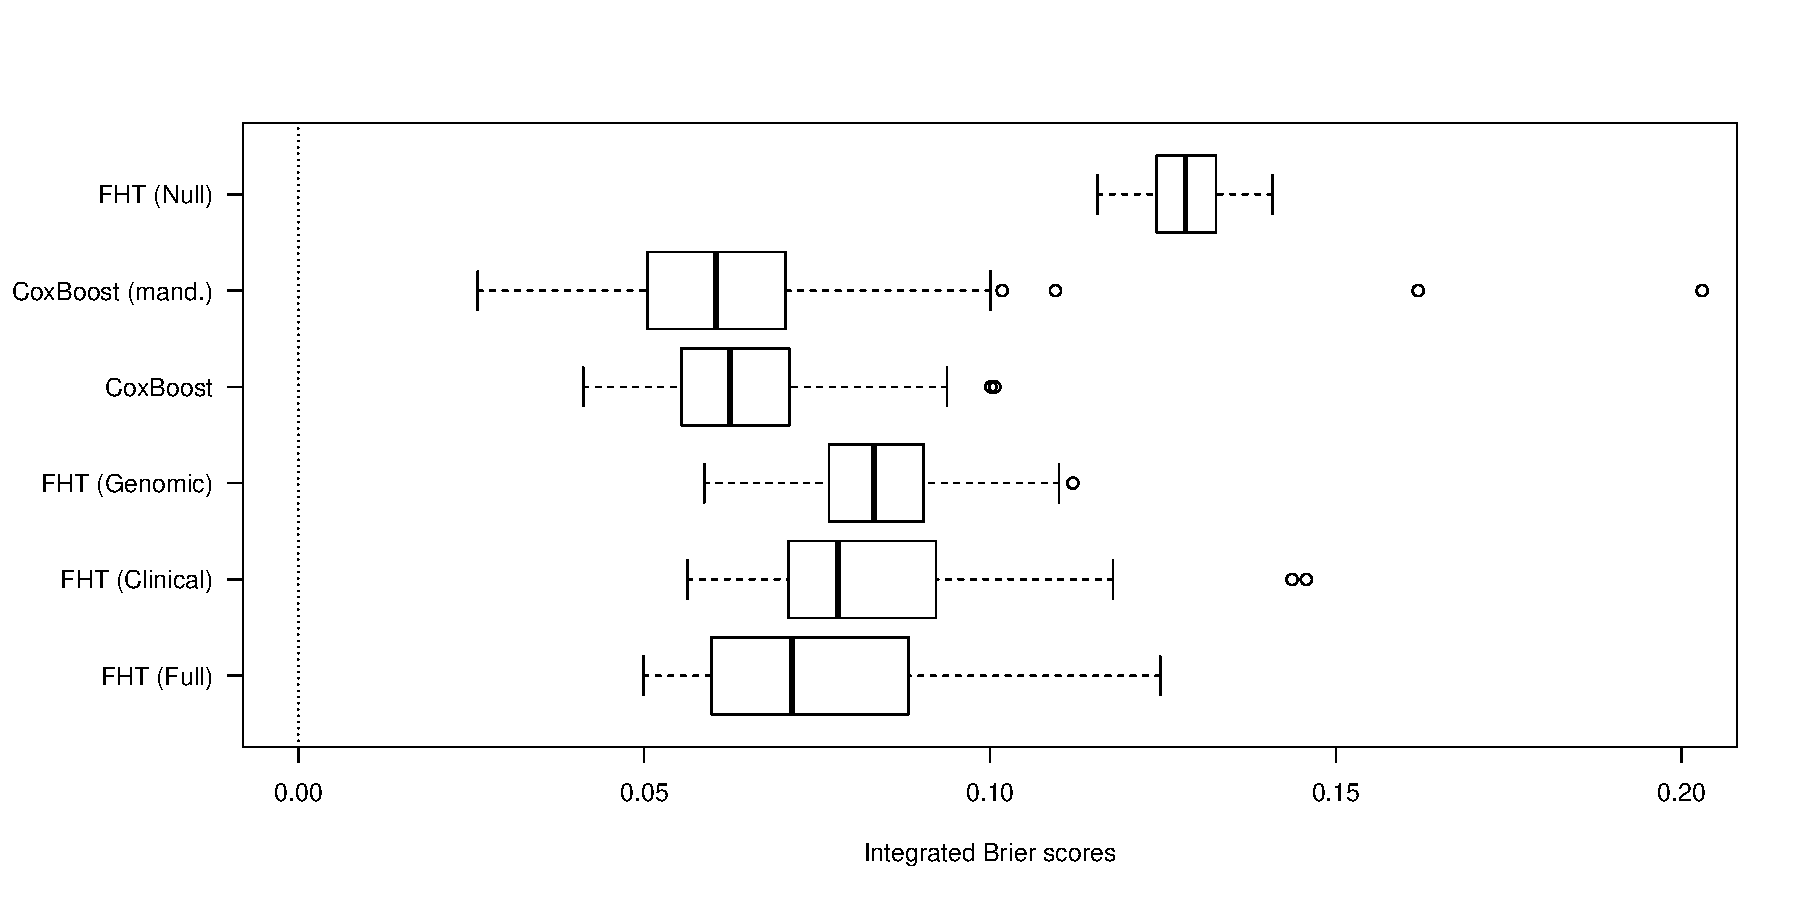
\includegraphics[scale=0.4]{integrated_brier_boxplot.pdf}
\end{figure}
With regard to this integrated Brier score, the full model performs slightly better than the clinical model.
It turns out that the full model performs slightly better than the clinical model, based on the median difference of deviance.
It might therefore appear as if the genomic data sometimes improves performance, and sometimes does not.
However, the genomic-only model vastly outperforms the full FHT model.
We get a median integrated Brier score of 3.9 for the full FHT model, only slightly beating the clinical one at 3.7.
The genomic model, however, achieves 6.8, whereas the Cox model performs best, at 7.7.

I'm not sure why this happens, especially since the log-likelihood of the full model is best.
It looks like the observations which improve the likelihood are not those which improve the Brier score.
If these were the same, then we would most likely see the same model perform best in both regards.
It might, for example, be, at least based on the example seen earlier, that the genomic model in this case better explains the later observations, whereas the clinical data is better at lifetimes of smaller value.

\section{Conclusion}
Applying the FHT model to this data set has been a partly fruitful effort.
The model is able to incorporate covariate information to improve the model fit.
However, the predictive power is quite off from the Cox model.

%\section{Colon cancer}
%We now consider data originating from \citet{marisa-data}, consisting of patients diagnosed with colon cancer.
%Colon cancer is the third most common cancer, and the fourth leading cause of cancer death worldwide \citep{marisa-data}.
%Pathological staging is the only prognostic

%The French national CIT program involves a multicenter cohort of 750 patients with stage I to IV CC.

%About the data.

%We remove observations where any covariate is missing.

%We have four clinical measurements.
%These are sex, which is coded as a dummy variable $x_{\text{sex}}\in\{-1,1\}$, age, subtype, and finally stage.

%In the original data set, some survival times are originally 0.
%We first tried setting these to $10^{-9}$, but it resulted in numerical instability when using numerical optimization to find the maximum likelihood intercepts.
%We then tried setting these successively to $10^{-9},\,10^{-8},\,\cdot$, and not until 0.1 did we achieve numerical stability.
%Note that this likely has a large effect on the estimated parameters.